
\documentclass[11pt,a4paper]{article}
\usepackage[spanish,es-noindentfirst]{babel}
\usepackage{geometry}
\geometry{margin=2.5cm}
\usepackage{graphicx}
\usepackage{booktabs}
\usepackage{longtable}
\usepackage{array}
\usepackage{hyperref}
\usepackage{xcolor}
\usepackage{caption}
\usepackage{amsmath}
\usepackage{amssymb}
\usepackage{enumitem}
\usepackage{fancyhdr}
\usepackage{titlesec}

\hypersetup{colorlinks=true, linkcolor=blue!50!black, citecolor=blue!50!black, urlcolor=blue!50!black}

\titleformat{\section}{\large\bfseries}{\thesection}{1em}{}
\titleformat{\subsection}{\normalsize\bfseries}{\thesubsection}{1em}{}

\pagestyle{fancy}
\fancyhf{}
\fancyhead[L]{\small Diseño in silico de oligonucleótidos antisentido para ABCA4 c.161-395G>A}
\fancyhead[R]{\small Informe de avance}
\fancyfoot[C]{\thepage}

\newcommand{\bloqueacolor}{teal}
\newcommand{\advcolor}{orange!80!black}

\title{\textbf{Diseño computacional de oligonucleótidos antisentido (PMO) contra la variante intrónica profunda ABCA4 c.161-395G>A: informe de avance metodológico}}
\author{
Sergio Mauricio Nuñez\thanks{Concepción del proyecto, diseño del pipeline, análisis computacional, redacción. \newline \textit{YAIS Lab.} Contacto: \href{mailto:mauricio.nunez@yaislab.org}{mauricio.nunez@yaislab.org}.}
\quad
Amyra Sanchez\thanks{Revisión de dominio, curación de literatura y revisión del manuscrito. \newline \textit{YAIS Lab.}}
\and
\textit{Con asistencia de agentes de IA (Claude, Anthropic) para implementación de software, ejecución de pipelines y redacción bajo supervisión de los autores.}
}
\date{30 de julio de 2026}

\begin{document}
\maketitle

\begin{abstract}
\noindent
La variante intrónica profunda \textbf{ABCA4 c.161-395G>A} genera un pseudoexón aberrante (PE1b, 91~pb) que introduce un codón de terminación prematuro, y está asociada a un subtipo de la enfermedad de Stargardt tipo~1. Presentamos un pipeline computacional reproducible, de siete módulos, para el diseño \emph{in silico} de candidatos a oligonucleótido antisentido (ASO) de química \textbf{PMO} (morfolino fosforodiamidato) dirigidos a bloquear este pseudoexón por impedimento estérico. A partir de 381 ventanas candidatas generadas por barrido exhaustivo, el filtrado heurístico y termodinámico redujo el conjunto a 44 candidatos. Usamos dos predictores de splicing basados en redes neuronales, entrenados por grupos independientes con arquitecturas distintas (SpliceAI, Illumina; Pangolin, U. Pennsylvania), para (i)~confirmar computacionalmente la existencia y coordenadas exactas del pseudoexón --- con una coincidencia exacta de tamaño (91~pb) contra un dato experimental de minigén publicado por Peng et al. (2025) --- y (ii)~simular in silico el bloqueo de cada uno de los 44 candidatos. Al reclasificar el efecto de bloqueo con el criterio biológicamente correcto (anular \emph{cualquiera} de los dos bordes de splicing del pseudoexón, no solo el sitio donador), ambos predictores concuerdan al 100\,\% (44/44) en identificar el mismo subconjunto de \textbf{10 candidatos} que desarman el pseudoexón sin dañar el splicing canónico del exón~3. Un ranking multicriterio por \textbf{frente de Pareto} --- sin pesos arbitrarios, dado que no existe control positivo con el cual calibrarlos --- reduce esos 10 a \textbf{3 candidatos no dominados}, cada uno representando un compromiso distinto entre las tres dimensiones evaluadas. Este informe documenta también las limitaciones metodológicas del trabajo --- ausencia de validación experimental, química PMO sin precedente publicado en esta variante, ausencia de modelado real de hibridación --- y deja el pipeline completo (7 de 7 módulos) para orientar el trabajo futuro y la búsqueda de financiamiento.
\end{abstract}

\tableofcontents

\section{Motivación y contexto biológico}

La enfermedad de Stargardt tipo~1 es la distrofia macular hereditaria más frecuente y está causada por variantes bialélicas en el gen \textbf{ABCA4}. Una fracción relevante de los alelos patogénicos no son variantes codificantes clásicas, sino \textbf{variantes intrónicas profundas} que activan sitios de splicing crípticos, generando la inclusión de un \emph{pseudoexón} --- una secuencia intrónica que la maquinaria de splicing trata erróneamente como un exón --- y con ello un codón de terminación prematuro que trunca la proteína.

La variante \textbf{c.161-395G>A} (confirmada en coordenadas genómicas GRCh38 mediante VariantValidator, con verificación cruzada independiente vía Ensembl) es una de estas variantes. Peng et al. (2025, \emph{IOVS}) demostraron experimentalmente, mediante ensayo de minigén, que esta variante activa un pseudoexón de \textbf{91~pb} (denominado PE1b en esa publicación), con 76{,}4\,\% del ARNm resultante empalmado incorrectamente.

Los ASOs de tipo \emph{splice-switching} son oligonucleótidos sintéticos que se unen por complementariedad de bases a una región del pre-ARNm y bloquean físicamente el acceso de la maquinaria de splicing a un sitio específico, sin degradar la molécula. Aplicados sobre un pseudoexón, pueden en principio restaurar el splicing normal. No existe, hasta donde este proyecto pudo verificar, ningún ASO publicado o patentado dirigido específicamente a esta variante o a sus pseudoexones (PE1b/PE1c/PE1d) --- una brecha que motiva este trabajo, pero que también significa que \textbf{no hay ningún resultado conocido contra el cual validar el pipeline de punta a punta}. Esta ausencia de control positivo termina siendo la limitación transversal que atraviesa todo el proyecto y que se declara en cada sección de resultados.

Se especificó por decisión de alcance del proyecto (no por evidencia clínica retinal específica) el uso de química \textbf{PMO}, cuyo esqueleto neutro y mecanismo de bloqueo estérico puro (sin activación de RNasa~H) la distingue de la química 2'-MOE/fosforotioato usada en los ASOs retinales con eficacia clínica publicada hasta la fecha (p.~ej. QR-1011).

\section{Pipeline y estado de avance}

El proyecto está organizado en siete módulos secuenciales, los \textbf{siete implementados y verificados} al momento de este informe.

\begin{center}
\begin{longtable}{@{}p{1.3cm}p{4.7cm}p{6.8cm}p{1cm}@{}}
\toprule
\textbf{Módulo} & \textbf{Función} & \textbf{Resultado clave} & \textbf{Estado} \\
\midrule
\endhead
1 & Adquisición y validación de secuencia genómica & Coordenada de variante y límites del intrón~2 (1393~nt) confirmados de forma independiente (VariantValidator + Ensembl) & \checkmark \\
2 & \emph{Oligo-Walk}: barrido exhaustivo de ventanas candidatas & 381 ventanas candidatas generadas sobre la región de interés & \checkmark \\
3 & Filtro heurístico (GC\%, \emph{G-runs}, motivos) & 381 $\rightarrow$ 276 candidatos sobreviven & \checkmark \\
4 & Termodinámica (ViennaRNA: $T_m$, $\Delta G$, accesibilidad) & 276 $\rightarrow$ \textbf{44} candidatos finales sobreviven & \checkmark \\
5 & Severidad off-target (BLAST+ contra transcriptoma humano) & 44/44 anotados con severidad (no descarte binario): 1 alto / 18 moderado / 18 leve / 7 sin señal & \checkmark \\
6/6b/6c & Validación neural de splicing y simulación de bloqueo (SpliceAI + Pangolin, validación cruzada) & \textbf{10/44} candidatos anulan el pseudoexón, con concordancia total entre predictores & \checkmark \\
7 & Ranking multicriterio final & Frente de Pareto sobre 3 dimensiones: 10 $\rightarrow$ \textbf{3} candidatos no dominados & \checkmark \\
\bottomrule
\end{longtable}
\end{center}

Todo el pipeline corre en tres entornos de software aislados (\texttt{bio-oligo}, \texttt{spliceai}, \texttt{pangolin}), documentados con \texttt{requirements} versionados y un \texttt{README} que especifica el comando exacto para regenerar cada resultado desde cero. La suite de pruebas automatizadas cubre 207 casos y pasa en su totalidad al momento de este informe.

\section{Métodos}

\subsection{Generación y filtrado de candidatos (Módulos 1--5)}

Sobre una ventana genómica de 12{,}001~nt centrada en la variante (6000~nt de contexto a cada lado, requeridos por el segundo predictor neuronal), se generaron 381 ventanas candidatas de longitud típica de un PMO (barrido exhaustivo, \emph{Oligo-Walk}). El filtro heurístico eliminó candidatos con contenido de GC fuera de rango o tramos homopoliméricos (\emph{G-runs}) que favorecen agregación. El filtro termodinámico, usando ViennaRNA sobre la secuencia de bases como aproximación (los parámetros \emph{nearest-neighbor} estándar no están calibrados para el esqueleto neutro del PMO --- limitación declarada explícitamente en el Módulo~4), evaluó temperatura de fusión, energía libre de plegamiento y accesibilidad relativa de la región blanco, dejando 44 candidatos.

El cribado de off-target (BLAST+ local contra el transcriptoma humano completo, cDNA+ncRNA de Ensembl GRCh38) inicialmente aplicó la regla binaria heredada de la literatura de \emph{gapmers} (ASOs que activan RNasa~H): «$\geq$15~pb de homología contigua con $\leq$4 \emph{mismatches} en otro gen $\rightarrow$ descartar». Aplicada tal cual, esa regla marcó a los 44/44 candidatos como tóxicos --- es decir, no discriminaba nada, porque fue diseñada para un mecanismo de corte enzimático que un PMO (que solo bloquea, no corta) no comparte. Se reemplazó por una anotación de \textbf{severidad} de cuatro niveles medida sobre el tramo contiguo perfecto más largo del alineamiento (no el conteo de \emph{mismatches}, que biofísicamente invierte el orden de riesgo real), dejando la severidad como insumo para el ranking del Módulo~7 en vez de un descarte automático.

\subsection{Validación neuronal de splicing y simulación de bloqueo (Módulos 6, 6b, 6c)}

Se usaron dos redes neuronales convolucionales de predicción de splicing, entrenadas independientemente por grupos distintos sobre datos y arquitecturas distintas: \textbf{SpliceAI} (Illumina, Jaganathan et al. 2019) y \textbf{Pangolin} (Zeng \& Li, 2022), ambas ejecutadas por inferencia local (sin GPU). Antes de interpretar cualquier predicción nueva se verificó, para cada predictor, que recupera los cuatro sitios de splicing canónicos ya conocidos por coordenadas independientes (exones~2 y~3) con scores $>0{,}95$ --- el primer control positivo real del proyecto.

\textbf{Simulación de bloqueo.} El efecto de un ASO se simuló reemplazando su ventana objetivo por el carácter \texttt{N} (base desconocida), que ambos predictores codifican como vector nulo --- una aproximación \emph{in silico} al bloqueo estérico físico de un PMO real, validada con cuatro controles (ventanas lejanas sin efecto, enmascarado del donador canónico que solo afecta ese sitio, invariancia frente al tamaño de la ventana de contexto, y verificación de que ambos predictores comparten la misma codificación de \texttt{N}).

\textbf{Criterio de clasificación (hallazgo metodológico central de este informe).} La primera versión del módulo clasificaba el efecto de cada candidato mirando únicamente la retención del score del \emph{sitio donador} críptico. Al comparar los dos predictores bajo ese criterio, la concordancia era de solo 35/44 (79{,}5\,\%). La investigación de esa discrepancia --- en vez de promediarla o ignorarla --- reveló que los 9 candidatos discordantes formaban un grupo biológicamente coherente: ventanas que \textbf{anulan el sitio aceptor} del pseudoexón sin cubrirlo físicamente (el aceptor cae sobre un tracto rico en pirimidinas, verificado en la secuencia real: 77--80\,\% de pirimidinas frente a 50\,\% en una ventana sin efecto), y que ambos predictores modelan como una caída correlacionada del score del donador --- consistente con que las redes aprenden los dos bordes de un exón como un par funcional, no como sitios independientes. La métrica correcta, biológicamente, no es ``¿se anuló el donador?'' sino \textbf{``¿se anuló el pseudoexón?''}: basta con anular \emph{cualquiera} de los dos bordes de splicing para que el pseudoexón deje de incluirse, con la condición de seguridad explícita de que el candidato no dañe el sitio donador canónico del exón~3 sano.

\subsection{Ranking multicriterio (Módulo 7)}

Los 10 candidatos que anulan el pseudoexón bajo ambos predictores se ordenaron combinando tres dimensiones, cada una proveniente de un módulo distinto: \textbf{fuerza de bloqueo} ($1$ menos la retención media del borde mejor anulado, promediando los dos predictores; Módulos~6b/6c), \textbf{seguridad off-target} (negativo del tramo contiguo perfecto más largo contra otro gen; Módulo~5) y \textbf{calidad termodinámica} (media de los percentiles de accesibilidad y de no-autodimerización, relativos a los 44 candidatos que compiten entre sí; Módulo~4).

\textbf{No se empleó una suma ponderada.} Las tres dimensiones tienen unidades incomparables --- una fracción de señal de splicing, una longitud en pares de bases, un percentil relativo --- y promediarlas exige postular una tasa de cambio entre ellas (cuántos pb de homología off-target ``valen'' $0{,}01$ de fuerza de bloqueo) que ningún dato de este trabajo respalda, precisamente por la ausencia de control positivo. Se calculó en cambio el \textbf{frente de Pareto}: el conjunto de candidatos que ningún otro supera simultáneamente en las tres dimensiones. Es una afirmación más débil, pero verificable.

La elegibilidad para el ranking no es una cuarta dimensión sino una condición de entrada: solo compiten los candidatos cuyo veredicto es ``anula el pseudoexón'' bajo \emph{ambos} predictores.

\section{Resultados}

\subsection{Confirmación computacional del pseudoexón y coincidencia con dato experimental}

SpliceAI predice que la variante c.161-395G>A activa un donador críptico en la posición $+1$ (score WT$\to$MU: 0{,}194$\to$0{,}560, $\Delta=+0{,}366$) y un aceptor críptico en $-89$ ($\Delta=+0{,}210$). El pseudoexón resultante mide \textbf{91~pb}, que coincide \emph{exactamente} con el tamaño de PE1b medido por ensayo de minigén en Peng et al. (2025) --- dos métodos completamente independientes (predicción computacional y medición experimental \emph{in vitro}) convergiendo en el mismo número. Pangolin, ejecutado sobre los mismos cuatro tejidos disponibles en el modelo, confirma el mismo par de sitios en el mismo orden de importancia relativa (donador $+1$: $\Delta=+0{,}209$; aceptor $-89$: $\Delta=+0{,}124$), constituyendo un segundo control independiente sobre el hallazgo central del proyecto.

\begin{figure}[htbp]
\centering
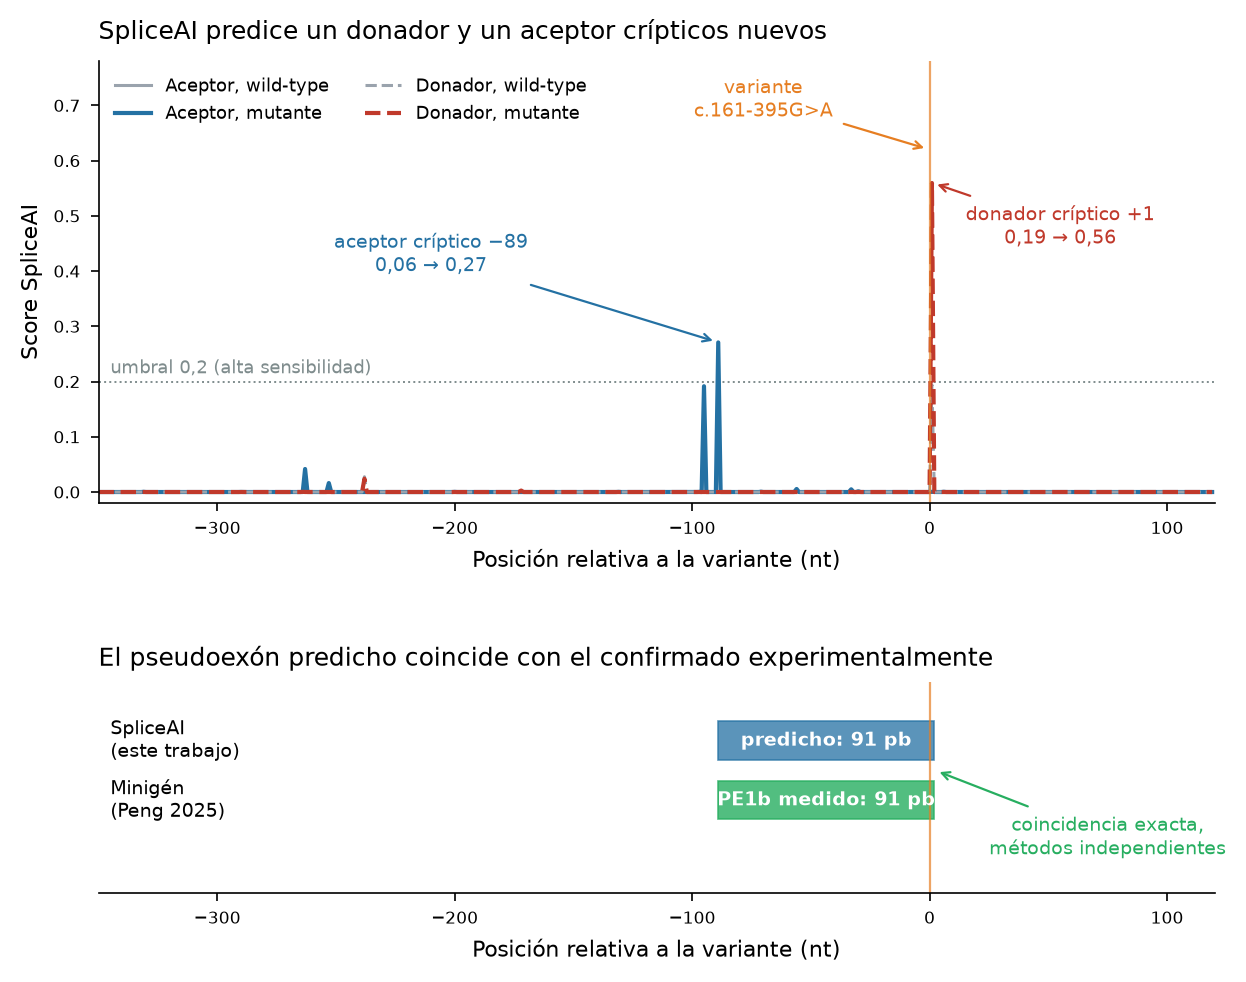
\includegraphics[width=0.85\textwidth]{figs/2026-07-30-spliceai-validacion-pe1b.png}
\caption{Predicción SpliceAI del donador y aceptor crípticos generados por la variante, y coincidencia exacta de tamaño (91~pb) con el pseudoexón PE1b medido experimentalmente por Peng et al. (2025).}
\end{figure}

\begin{figure}[htbp]
\centering
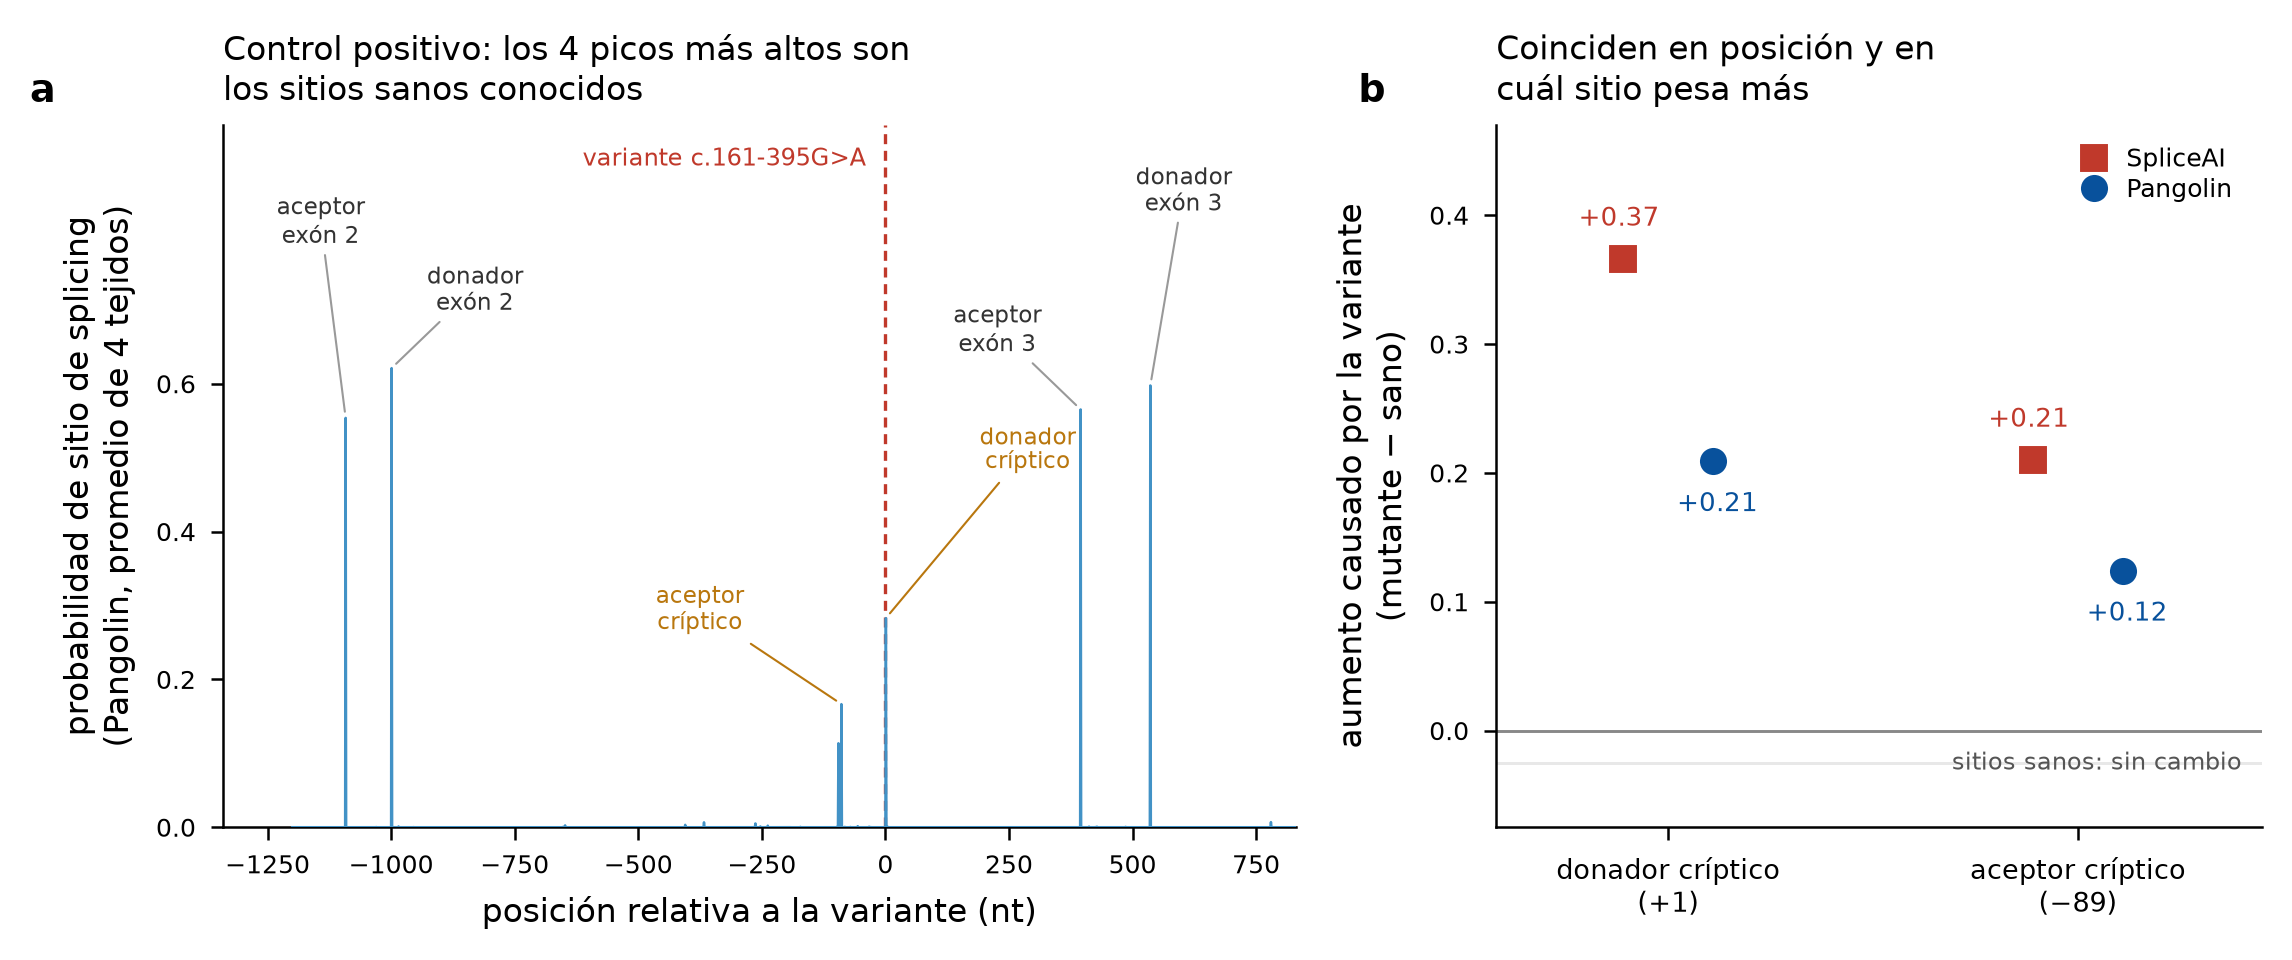
\includegraphics[width=0.95\textwidth]{figs/2026-07-30-pangolin-validacion.png}
\caption{Validación cruzada con Pangolin: recupera los cuatro sitios canónicos como los picos de mayor score de todo el perfil, y coincide con SpliceAI en la posición e importancia relativa de los dos sitios crípticos.}
\end{figure}

\subsection{Simulación de bloqueo: 10 candidatos anulan el pseudoexón con concordancia total}

De los 44 candidatos, \textbf{10} (22{,}7\,\%) producen el veredicto \emph{anula el pseudoexón} bajo el criterio de dos bordes, y en los 10 casos el sitio donador canónico del exón~3 sano queda intacto (retención $\approx$1{,}00--1{,}07 respecto del \emph{baseline}, en ambos predictores). Tres de ellos cubren físicamente el sitio donador críptico y lo anulan por completo (retención $=0{,}000$ en ambos predictores); los otros siete no cubren el aceptor críptico pero igualmente lo anulan (retención 0{,}45--0{,}59 en SpliceAI, 0{,}15--0{,}35 en Pangolin), consistente con el mecanismo de tracto de polipirimidina descrito arriba.

\begin{center}
\begin{longtable}{@{}p{2.1cm}p{1.6cm}p{2.3cm}p{2cm}p{2cm}p{2cm}p{2cm}@{}}
\toprule
\textbf{Candidato} & \textbf{Posición} & \textbf{Borde(s) anulado(s)} & \textbf{Ret. donador (S)} & \textbf{Ret. donador (P)} & \textbf{Ret. aceptor (S)} & \textbf{Ret. aceptor (P)} \\
\midrule
\endhead
cand\_5877 & $-123$/$-103$ & aceptor & 0,537 & 0,178 & 0,077 & 0,034 \\
cand\_5878 & $-122$/$-102$ & aceptor & 0,529 & 0,170 & 0,045 & 0,013 \\
cand\_5879 & $-121$/$-101$ & aceptor & 0,521 & 0,178 & 0,012 & 0,003 \\
cand\_5880 & $-120$/$-100$ & aceptor & 0,501 & 0,156 & 0,021 & 0,004 \\
cand\_5881 & $-119$/$-99$ & aceptor & 0,458 & 0,155 & 0,036 & 0,011 \\
cand\_5882 & $-118$/$-98$ & aceptor & 0,532 & 0,218 & 0,009 & 0,003 \\
cand\_5883 & $-117$/$-97$ & aceptor & 0,589 & 0,353 & 0,016 & 0,006 \\
cand\_5992 & $-8$/$+12$ & donador+aceptor & 0,000 & 0,000 & 0,197 & 0,096 \\
cand\_5998 & $-2$/$+18$ & donador+aceptor & 0,000 & 0,000 & 0,164 & 0,073 \\
cand\_5999 & $-1$/$+19$ & donador+aceptor & 0,000 & 0,000 & 0,131 & 0,061 \\
\bottomrule
\end{longtable}
\captionof{table}{Los 10 candidatos que anulan el pseudoexón bajo ambos predictores (S~=~SpliceAI, P~=~Pangolin). Posición relativa a la variante, en nt. Retención = score enmascarado / score \emph{baseline} sin ASO; valores bajos indican bloqueo efectivo.}
\end{center}

\begin{figure}[htbp]
\centering
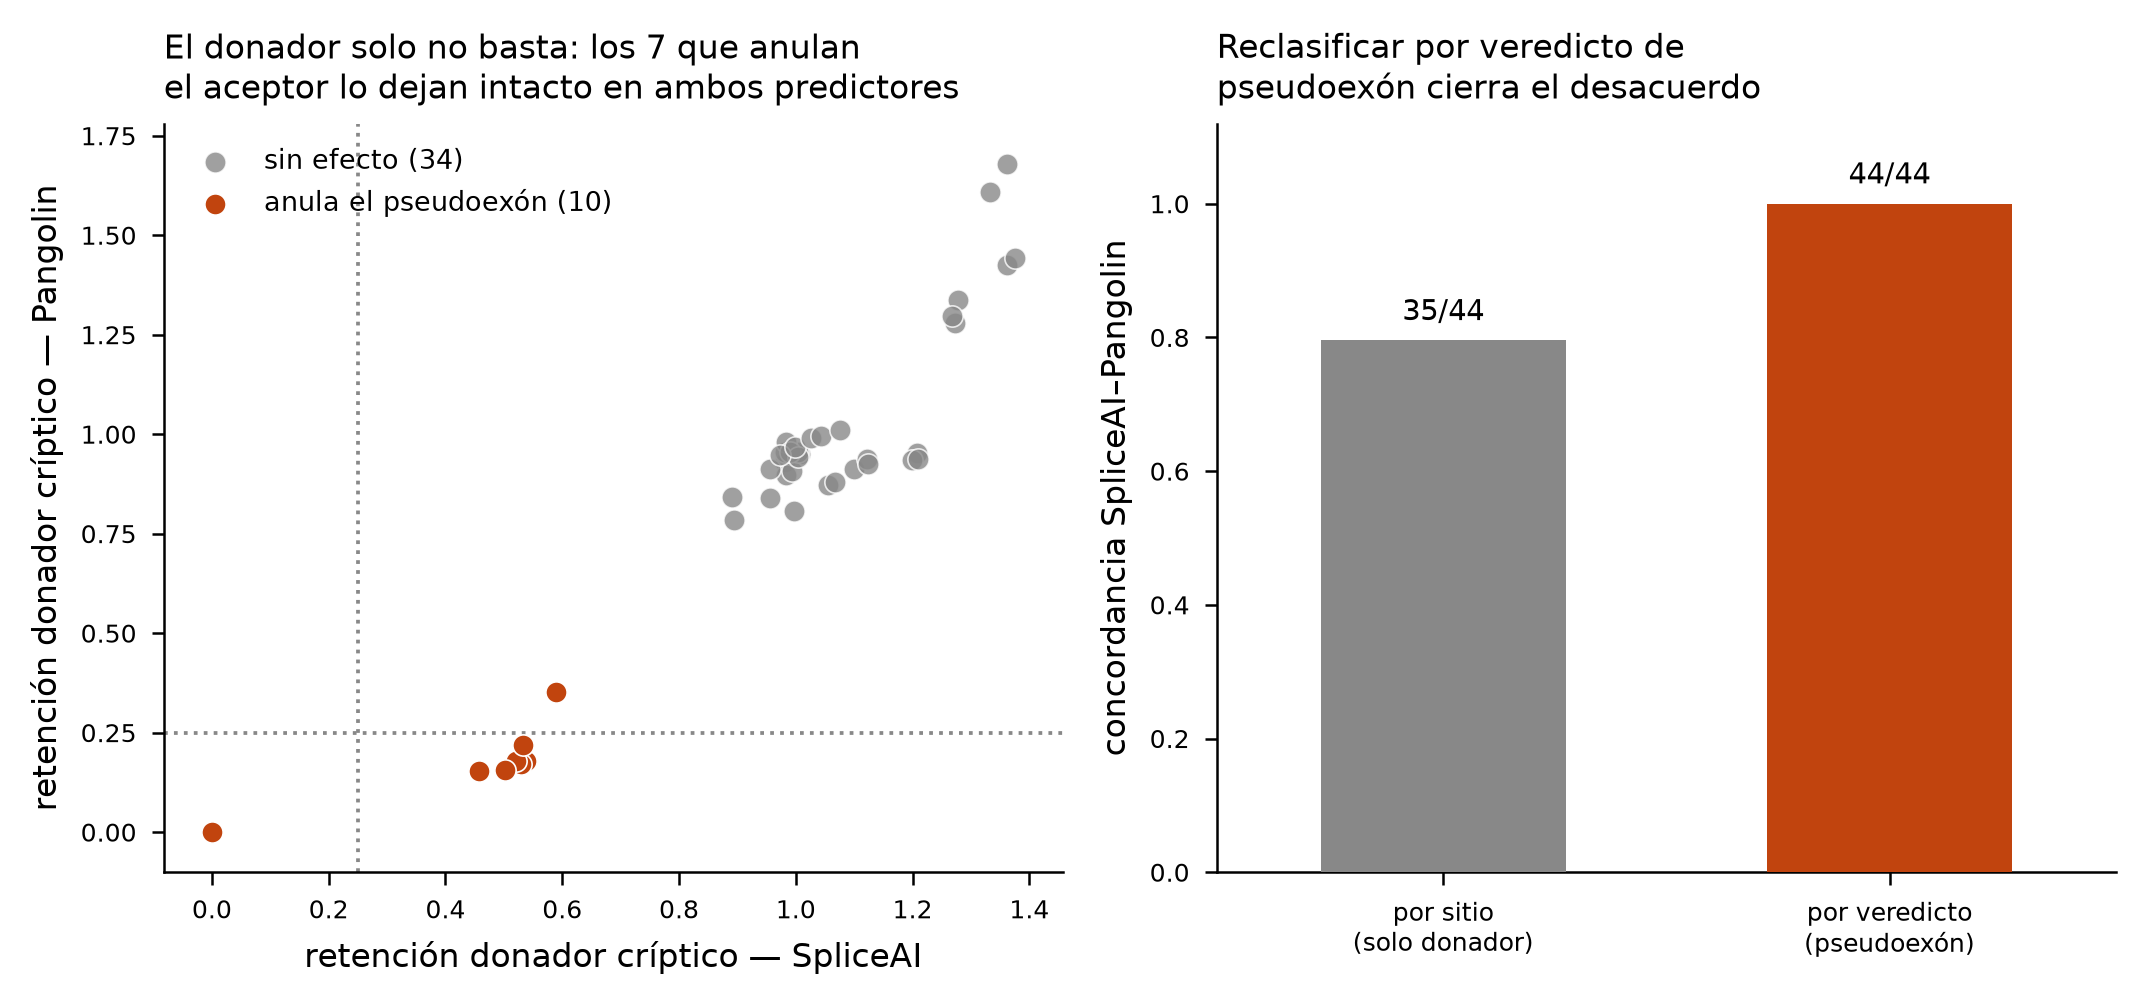
\includegraphics[width=\textwidth]{figs/concordancia_predictores_masking.png}
\caption{Concordancia entre predictores. \textbf{Izquierda:} retención del donador críptico, SpliceAI vs.\ Pangolin, para los 44 candidatos; los 7 candidatos que anulan el aceptor sin cubrirlo (rojo) muestran una caída correlacionada mas parcial del donador en ambos predictores. \textbf{Derecha:} la concordancia sube de 35/44 (79{,}5\,\%, criterio de un solo sitio) a 44/44 (100\,\%, criterio de veredicto a nivel pseudoexón) al reclasificar con la métrica biológicamente correcta.}
\end{figure}

\subsection{Severidad off-target}

Sobre los 44 candidatos completos (no solo los 10 que anulan el pseudoexón), la anotación de severidad off-target --- medida sobre el tramo contiguo perfecto más largo de homología con cualquier otro gen del transcriptoma humano --- distribuye así: 1 candidato de severidad alta ($\geq$18~pb contiguos), 18 moderada (16--17~pb), 18 leve (13--15~pb) y 7 sin señal ($\leq$12~pb). Esta anotación queda como insumo para el criterio de ranking del Módulo~7, no como filtro de descarte, dado que el mecanismo de bloqueo estérico de un PMO no comparte la lógica de destrucción del transcrito de los \emph{gapmers} que motivó la regla de corte original en la literatura.

\begin{figure}[htbp]
\centering
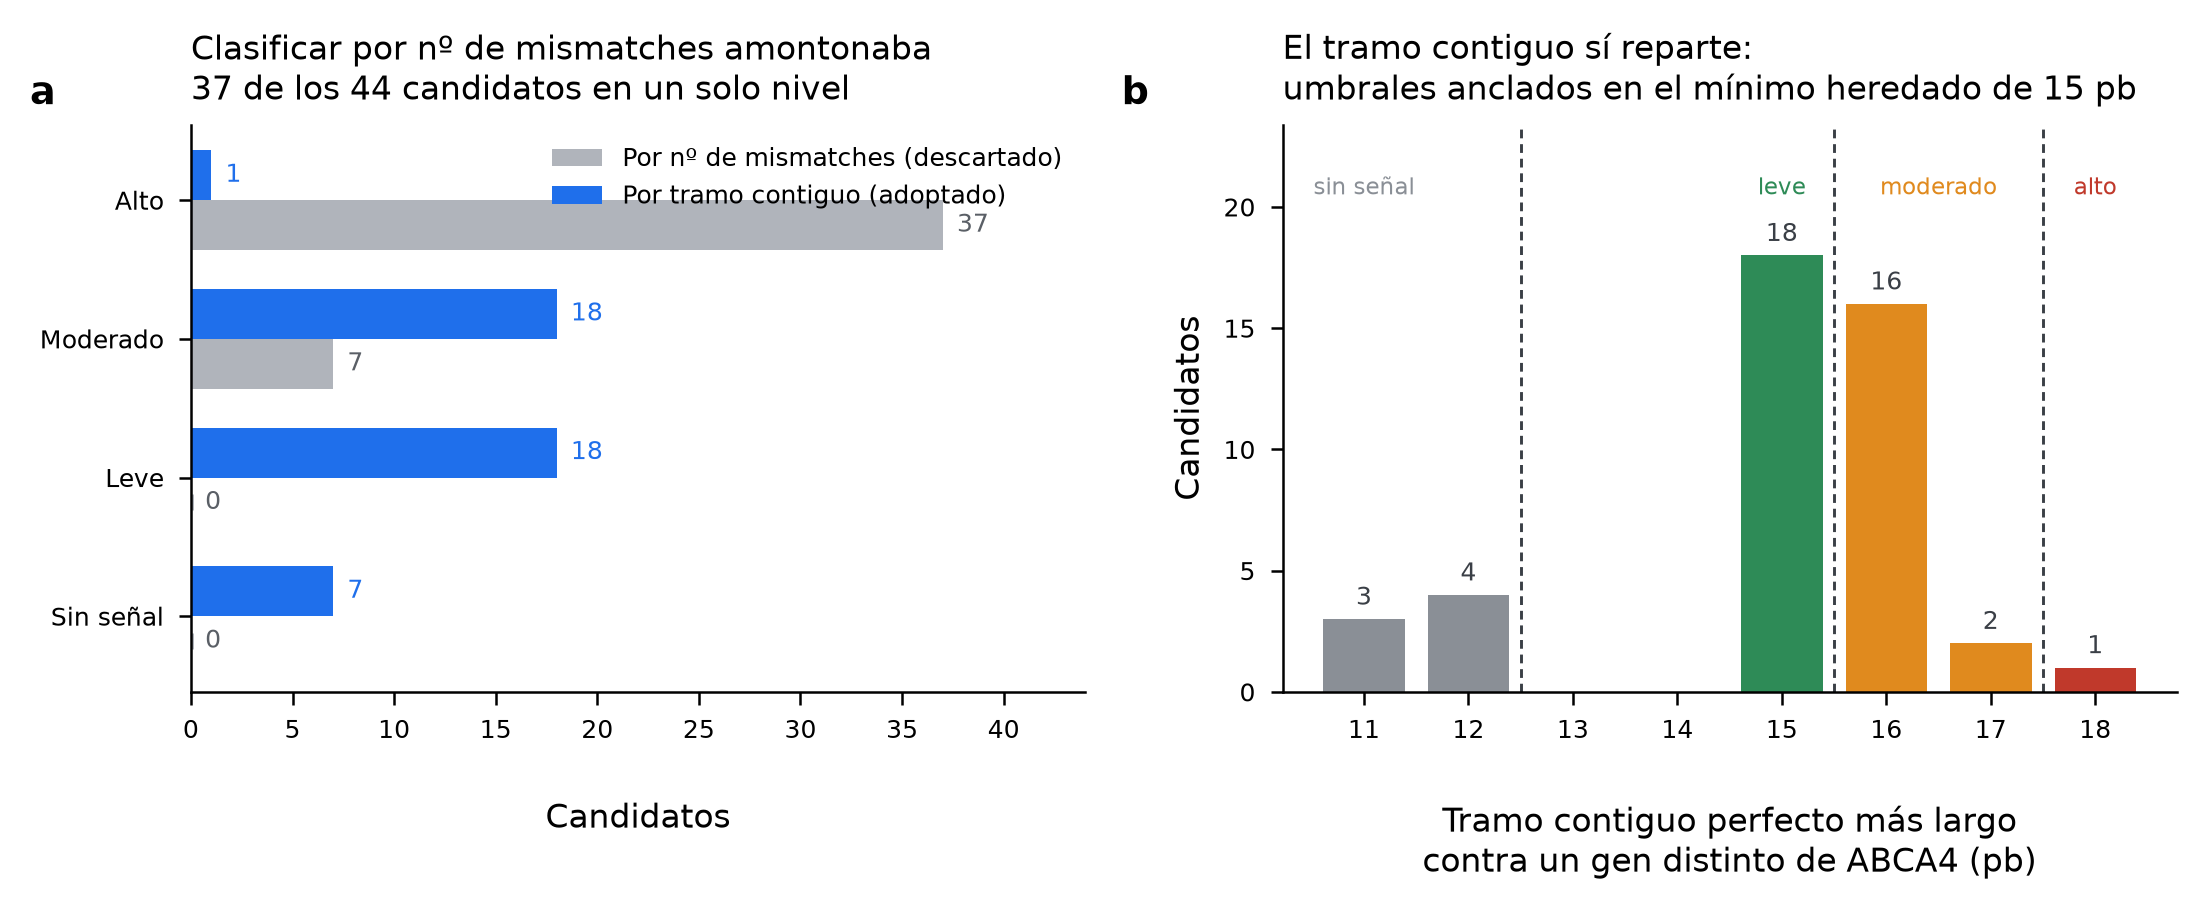
\includegraphics[width=\textwidth]{figs/2026-07-30-severidad-off-target-comparacion.png}
\caption{Comparación entre clasificar severidad off-target por número de \emph{mismatches} (izquierda, degenerado: 37/44 candidatos caen en un solo nivel) y por tramo contiguo perfecto más largo (derecha, criterio adoptado, con distribución no degenerada).}
\end{figure}

\subsection{Ranking final: tres candidatos no dominados, sin ganador único}

El frente de Pareto reduce los 10 candidatos elegibles a \textbf{3 no dominados} (Tabla~\ref{tab:pareto}). Ninguno domina a los otros dos: cada uno representa un compromiso distinto.

\begin{center}
\begin{longtable}{@{}llrrr@{}}
\toprule
\textbf{Candidato} & \textbf{Bordes anulados} & \textbf{Bloqueo} & \textbf{Off-target} & \textbf{Termodinámica} \\
\midrule
\endhead
\texttt{cand\_5992} & donador + aceptor & \textbf{1{,}00000} & 15~pb & 11{,}7 \\
\texttt{cand\_5998} & donador + aceptor & 0{,}99995 & 16~pb & 14{,}0 \\
\texttt{cand\_5882} & aceptor & 0{,}99420 & 15~pb & \textbf{65{,}2} \\
\bottomrule
\caption{Los 3 candidatos del frente de Pareto. Bloqueo: $1-$retención media del borde mejor anulado. Off-target: tramo contiguo perfecto más largo contra otro gen (menor es mejor). Termodinámica: percentil medio, relativo a los 44 candidatos (mayor es mejor).}
\label{tab:pareto}
\end{longtable}
\end{center}

\texttt{cand\_5992} maximiza el bloqueo, \texttt{cand\_5882} la calidad termodinámica, y \texttt{cand\_5998} \textbf{no maximiza ninguna dimensión individualmente} pero tampoco es superado en las tres a la vez --- el caso que un ordenamiento por columna única habría descartado, y que justifica el enfoque.

\textbf{Tensión estructural entre bloqueo y calidad de oligo.} Los tres candidatos que anulan \emph{ambos} bordes del pseudoexón (\texttt{cand\_5992}, \texttt{cand\_5998}, \texttt{cand\_5999}) son exactamente los tres peores en calidad termodinámica (percentiles $11{,}7$, $14{,}0$ y $9{,}3$), con una brecha de más de 26 puntos respecto del cuarto ($40{,}7$). Bloquear con mayor eficacia y ser mejor oligo fisicoquímicamente apuntan en direcciones opuestas. Este conflicto ya había sido detectado en el Módulo~4 entre accesibilidad estructural y proximidad al mecanismo; su reaparición por una vía independiente --- ahora sobre el efecto de bloqueo simulado, no sobre la distancia a la variante --- hace menos plausible que sea un artefacto de una sola métrica.

\textbf{Análisis de sensibilidad.} Colapsar accesibilidad y no-autodimerización en un único promedio constituye, en sí mismo, una ponderación implícita $50/50$. Se cuantificó su efecto: tratándolas como dimensiones separadas (cuatro objetivos en lugar de tres), el frente se ensancha de 3 a \textbf{9 de los 10} candidatos, es decir, deja de discriminar. La convención se adopta explícitamente por ser la que permite que el módulo informe, y se declara como tal en la salida de la API y en la interfaz, en lugar de quedar implícita en el código.

En consecuencia, \textbf{el pipeline no emite un ganador único}. Seleccionar uno de los tres exige decidir qué dimensión se prioriza, decisión que con la evidencia disponible corresponde al criterio experimental y no al cálculo.

\section{Limitaciones metodológicas}

Estas limitaciones se declaran explícitamente porque condicionan qué se puede afirmar con este trabajo y qué no:

\begin{enumerate}[leftmargin=*]
\item \textbf{Ninguna validación experimental.} Todos los resultados son predicciones computacionales. No se ha sintetizado, transfectado ni ensayado ningún ASO. La confirmación con el dato de Peng et al. (2025) valida la \emph{predicción del pseudoexón}, no el diseño del ASO ni su eficacia.
\item \textbf{Química PMO sin precedente publicado en esta variante o en retina.} Todos los ASOs retinales de ABCA4 con eficacia medida publicada hasta la fecha usan química 2'-MOE/fosforotioato, no PMO. La elección de PMO fue una decisión de alcance del proyecto, no una elección respaldada por evidencia clínica retinal específica.
\item \textbf{Ausencia de control positivo para el ASO en sí.} No existe ningún ASO publicado ni patentado contra esta variante específica. Los controles positivos obtenidos (recuperación de los 4 sitios canónicos; coincidencia de 91~pb con el dato de minigén) validan las capas predictivas del pipeline, no el diseño final del oligonucleótido.
\item \textbf{El enmascarado por \texttt{N} es una aproximación, no una simulación física.} No modela hibridación real, afinidad de unión, ocupación parcial, cinética ni contexto celular (núcleo, complejo de splicing ensamblándose en tiempo real). Es una hipótesis computacional pendiente de ensayo.
\item \textbf{Los parámetros termodinámicos (ViennaRNA) están calibrados para ADN/ARN con carga, no para el esqueleto neutro del PMO.} Se usan como aproximación basada en secuencia de bases, explícitamente declarada como tal.
\item \textbf{Ningún predictor modela retina específicamente}, ni el contexto tisular real donde debe actuar el ASO terapéutico.
\item \textbf{El Módulo 7 (ranking multicriterio) no está completo al momento de este informe.} Los 10 candidatos identificados aquí son candidatos \emph{viables} bajo el criterio de bloqueo del pseudoexón; todavía no están priorizados entre sí por un criterio multicriterio explícito que combine severidad off-target, termodinámica y fuerza de bloqueo.
\end{enumerate}

\section{Próximos pasos}

Con los siete módulos implementados, el trabajo restante ya no es computacional. El paso crítico para elevar el nivel de evidencia es la \textbf{validación experimental \emph{in vitro}} --- ensayo de minigén o células portadoras del alelo patogénico --- de al menos uno de los tres candidatos del frente de Pareto. Dado que el pipeline no los ordena entre sí, la elección de cuál sintetizar primero es una decisión experimental: \texttt{cand\_5992} representa la apuesta por máximo bloqueo, y \texttt{cand\_5882} la apuesta por mejores propiedades fisicoquímicas.

En paralelo, tres líneas mejorarían la calidad de la evidencia sin requerir laboratorio: (i)~calibrar los umbrales de severidad off-target contra datos de efectos fuera de diana mediados por hibridación en ASOs de \emph{splice-switching} (p.~ej. Scharner et al., 2020); (ii)~cuantificar el solapamiento entre los conjuntos de entrenamiento de SpliceAI y Pangolin, para establecer en qué medida su concordancia constituye evidencia independiente; y (iii)~esclarecer por qué el modelo explica PE1b pero no PE1c ni PE1d, los otros dos pseudoexones reportados para esta variante.

\section{Disponibilidad de código y reproducibilidad}

El pipeline completo, los tres entornos de software con sus \texttt{requirements} versionados, la documentación de arquitectura (\emph{Architecture Decision Records}) y la bitácora completa de decisiones y hallazgos están disponibles en el repositorio del proyecto. Cada resultado numérico presentado en este informe es regenerable con un comando documentado en el \texttt{README} del repositorio, sin dependencias de red no cacheadas (la secuencia genómica de referencia se almacena localmente con verificación de integridad por \emph{checksum}).

\vspace{1em}
\noindent\textit{Nota sobre método de trabajo: el desarrollo de software, la ejecución de los pipelines computacionales y la redacción de este informe se realizaron con asistencia de agentes de inteligencia artificial (Claude, Anthropic), bajo supervisión directa y decisión final de los autores en toda interpretación biológica y toda decisión de diseño. Las limitaciones listadas en la Sección~5 fueron mantenidas como requisito explícito de este proceso de trabajo.}

\end{document}
